\documentclass{standalone}
\usepackage{tikz}

\usetikzlibrary{shapes,arrows,fit,calc,positioning}
\usetikzlibrary{backgrounds}
\tikzstyle{input} = [coordinate]
\tikzstyle{output} = [coordinate]
\tikzstyle{box} = [draw, rectangle, fill=white, rounded corners, thick, node distance=10em, text width=7em, text centered, minimum height=5em]
\tikzstyle{container} = [draw, rectangle, dashed, inner sep=1em, node distance=5em]
\tikzstyle{line} = [draw, thick, -latex']
\begin{document}
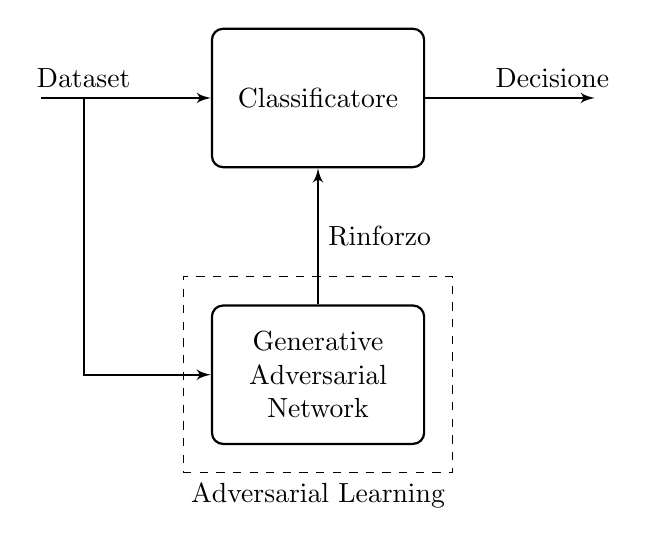
\begin{tikzpicture}[auto, node distance=10em]
	\node [input](input){};
	\node [box, right of=input](clas){Classificatore};
	\node [box, below of=clas](gan){Generative Adversarial Network};
	\node [container, fit=(gan)](adv){};
	\node at (adv.south) [below,node distance=0 and 0] {Adversarial Learning};	
	\node [output, right of=clas](output){};
		
	
	\path [line] (input) -- node[near start](dataset){Dataset} (clas);
	\path [line] (dataset) |- (gan);
	\path [line] (gan) -- node[right]{Rinforzo} (clas);
	\path [line] (clas) -- (output)node[near end,name=out]{Decisione};
\end{tikzpicture}
\end{document}